% Author: Dr. Matthias Jung, DL9MJ
% Year: 2020
\documentclass[convert = false, border=5pt]{standalone}
\usepackage{fontspec}
\setmainfont{Roboto}
\usepackage[siunitx, straightvoltages]{circuitikzgit}
\usepackage{tikz}


\begin{document}
	{
        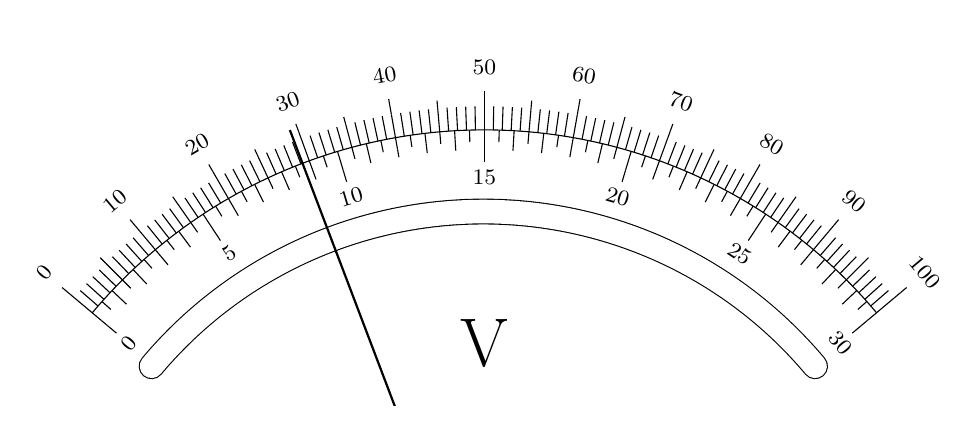
\begin{tikzpicture}
            % Beschneiden
            \clip[] (-5.8,7.8) rectangle (+5.8,3);
            % Obere Skala
            \foreach \b in {-50,-49,...,50}
                \edef\c{90 - \b * 1}
                \draw[] (\c:6.5) -- (\c:6.8);
            \foreach \b in {-50,-45,...,50}
                \edef\c{90 - \b * 1}
                \draw[] (\c:6.8) -- (\c:6.9);
            \foreach \b in {-50,-40,...,50}
                \edef\c{90 - \b * 1}
                \draw[] (\c:6.9) -- (\c:7);
            \foreach \b in {-50,-40,...,50}
                \edef\c{90 - \b * 1}
                \pgfmathtruncatemacro\result{abs(\b+50)}
                \draw (\c:7.3) node[rotate=\c-90] {\footnotesize\result};
            % Kreisbogen:
            \draw[] (4.98,4.18) arc (40:140:6.5);
            \draw[double distance = 0.3cm,line cap=round] (4.2,3.5) arc (40:140:5.5);
            % Untere Skala:
            \foreach \b in {-30,-29,...,30}
                \edef\c{90 - \b * 1.6666666}
                \draw[] (\c:6.5) -- (\c:6.35);
            \foreach \b in {-30,-28,...,30}
                \edef\c{90 - \b * 1.6666666}
                \draw[] (\c:6.35) -- (\c:6.25);
            \foreach \b in {-30,-20,...,30}
                \edef\c{90 - \b * 1.6666666}
                \draw[] (\c:6.25) -- (\c:6.10);
            \foreach \b in {-30,-20,...,30}
                \edef\c{90 - \b * 1.6666666}
                \pgfmathtruncatemacro\result{abs((\b+30)/2)}
                \draw (\c:5.9) node[rotate=\c-90] {\footnotesize\result};
            % Zeiger:
            \draw[thick] (0,0) -- (-2.47,6.5);
            % V:
            \draw (0,3.8) node[] {\Huge{V}};
        \end{tikzpicture}
    }
\end{document}
